\documentclass{beamer}
\usetheme{Mystyle}
\begin{document}
\begin{CJK*}{UTF8}{gkai}
  \title{十月}
  \author[\textcolor{black}{作者 朱海文}]{作者~~\textcolor{olive}{朱海文}}
  \institute{\textcolor{violet}{摩科特医疗器械有限公司}}
  \date{\today}
  \frame{\titlepage}
  %======================================================
  \section*{目录}
  \frame{\frametitle{目录}\tableofcontents}
  \section{一块探测器的模拟结果}
  \begin{frame}\frametitle{探测器晶粒几何}
    \begin{minipage}[t]{0.3\textwidth}
      \liuhao
      探测器晶粒共$24\times24$块,如果将中间的两块小晶粒合并成一块,则有
      $24\times16$块,列数为0-17列的
      即为合并之后的结果,事例数为($3.6\times10^8$)。
      
      晶粒编号从左至右为第i列($0\leq i \leq 25$),从上至下为
      第j行($100\le j \le2400$),在保存的时候将行数乘以100,以便区分行和列。
    \end{minipage}
    \begin{minipage}[t]{0.7\textwidth}
      \begin{figure}[ht]
	\centering
        \includegraphics[width=0.9\textwidth,height=0.7\textwidth]{Detector.png}
	\caption{\liuhao 探测器晶粒}
	\label{Detector}
      \end{figure}
    \end{minipage}
  \end{frame}
  %----------------------------
  \begin{frame}\frametitle{无准直器}
    \begin{figure}[ht]
      \centering
      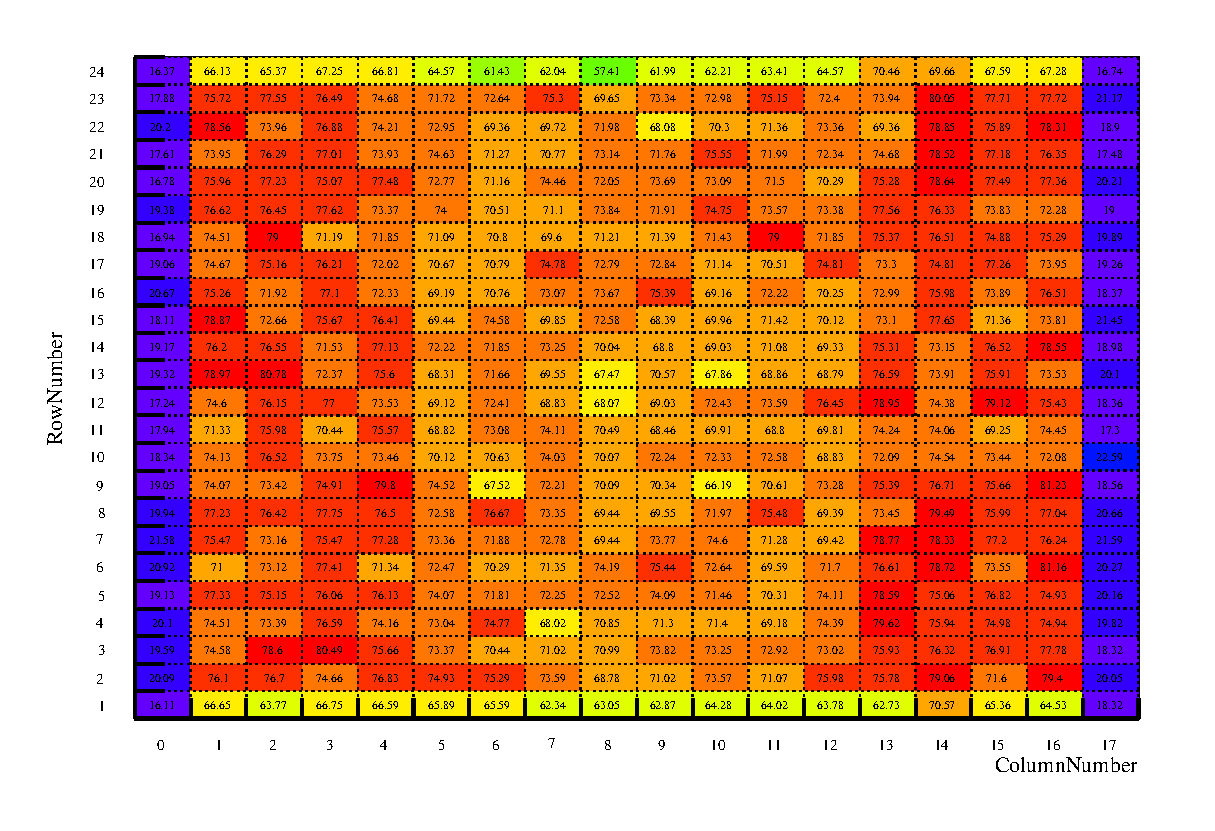
\includegraphics[width=\textwidth]{WithoutCollimatorDirectEnergyMerged.eps}
      \caption{\liuhao 无准直器时直射的能量(MeV)}
    \end{figure}
  \end{frame}
  %----------------------------
  \begin{frame}\frametitle{无准直器}
    \begin{figure}[ht]
      \centering
      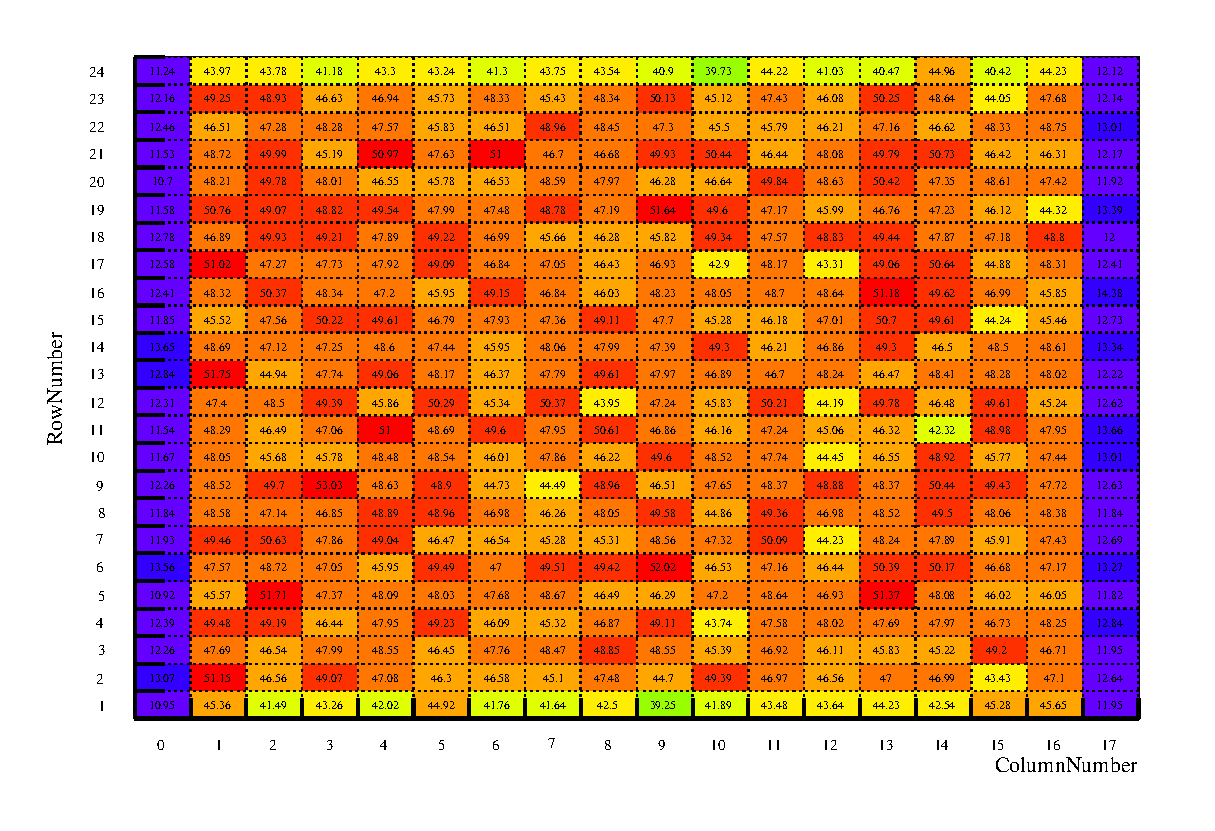
\includegraphics[width=\textwidth]{WithoutCollimatorScatteringEnergyMerged.eps}
      \caption{\liuhao 无准直器时散射的能量(MeV)}
    \end{figure}
  \end{frame}
  %----------------------------
  \begin{frame}\frametitle{无准直器}
    \begin{figure}[ht]
      \centering
      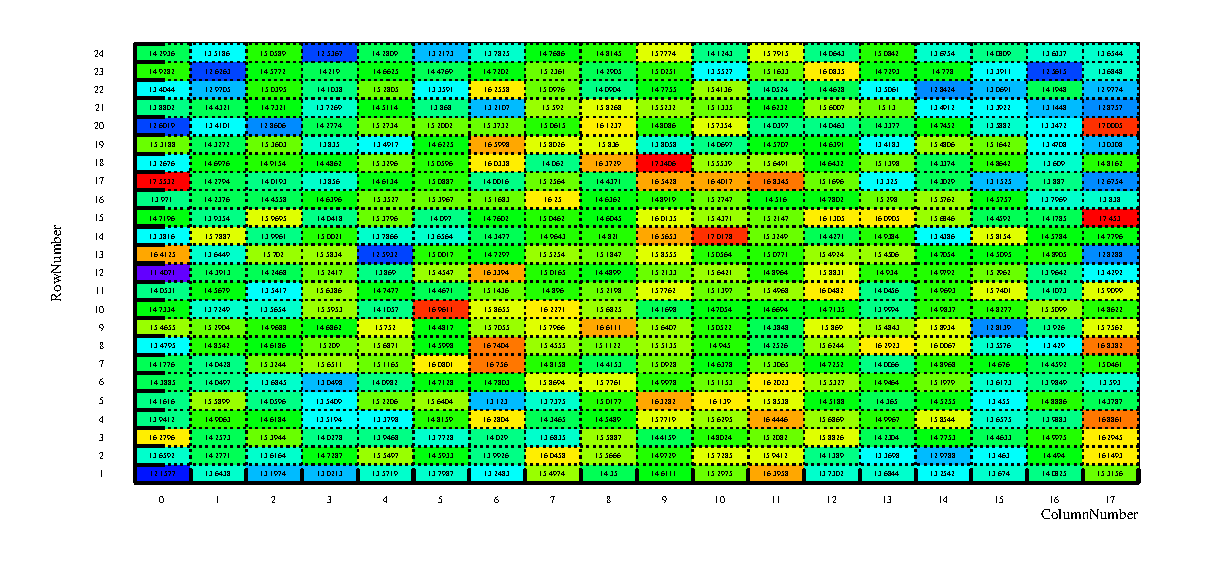
\includegraphics[width=\textwidth]{WithoutCollimatorScatteringRatioMerged.eps}
      \caption{\liuhao 无准直器时散射的比例(\%)}
    \end{figure}
  \end{frame}
 %----------------------------
  \begin{frame}\frametitle{有准直器}
    \begin{figure}[ht]
      \centering
      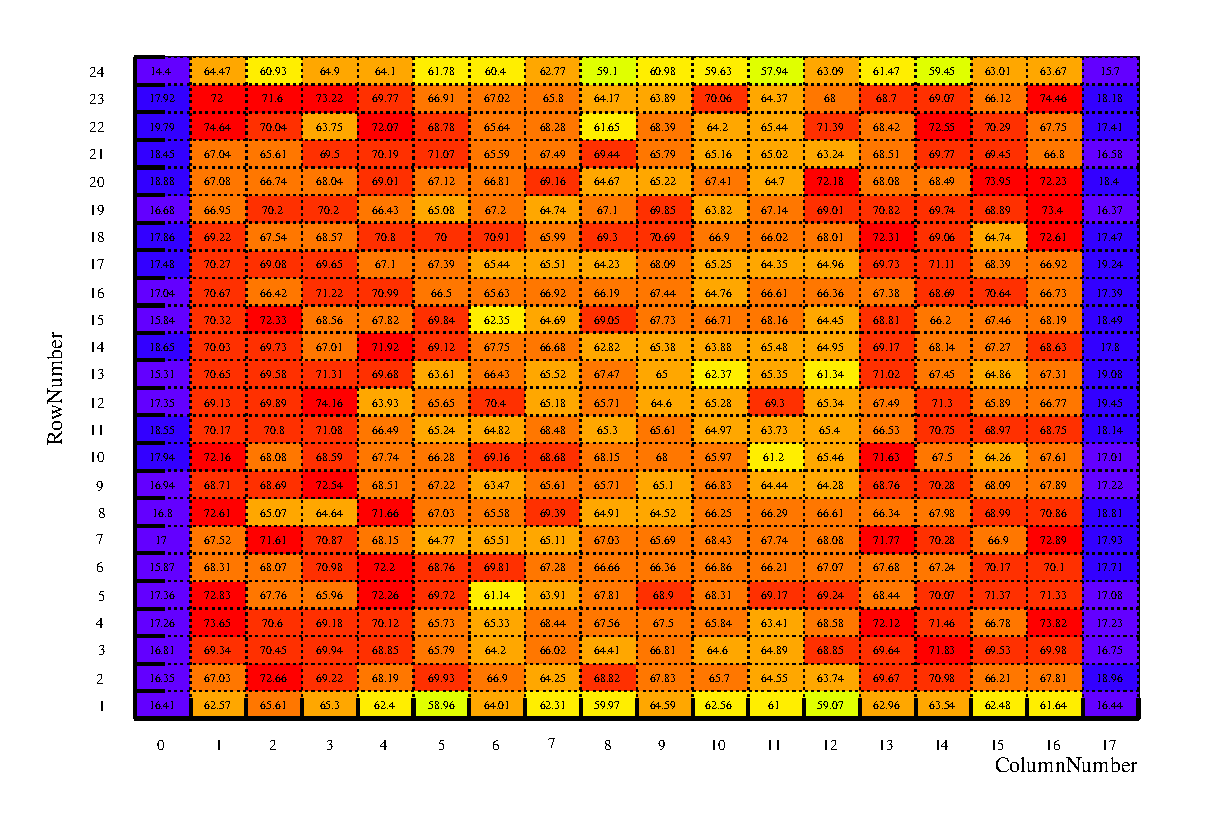
\includegraphics[width=\textwidth]{WithCollimatorDirectEnergyMerged.eps}
      \caption{\liuhao 有准直器时直射的能量(MeV)}
    \end{figure}
  \end{frame}
  %----------------------------
  \begin{frame}\frametitle{有准直器}
    \begin{figure}[ht]
      \centering
      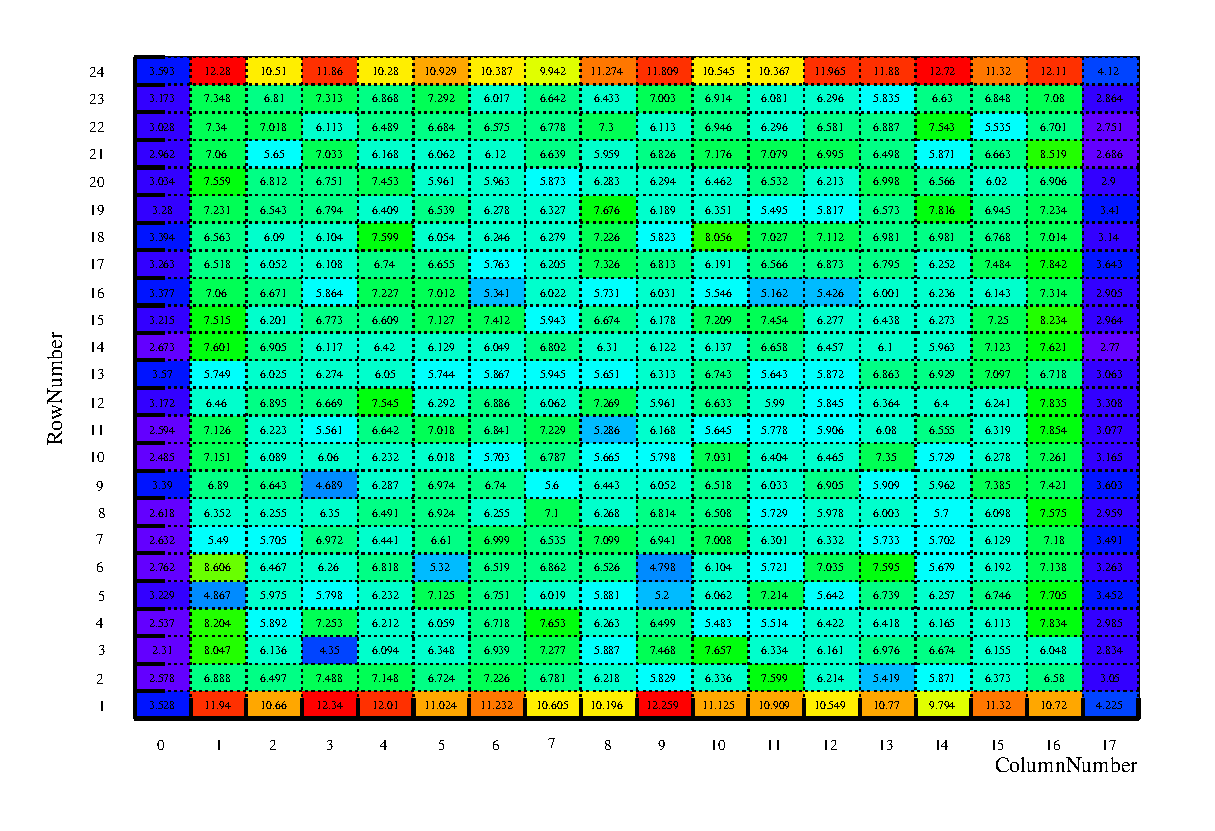
\includegraphics[width=\textwidth]{WithCollimatorScatteringEnergyMerged.eps}
      \caption{\liuhao 有准直器时散射的能量(MeV)}
    \end{figure}
  \end{frame}
  %----------------------------
  \begin{frame}\frametitle{有准直器}
    \begin{figure}[ht]
      \centering
      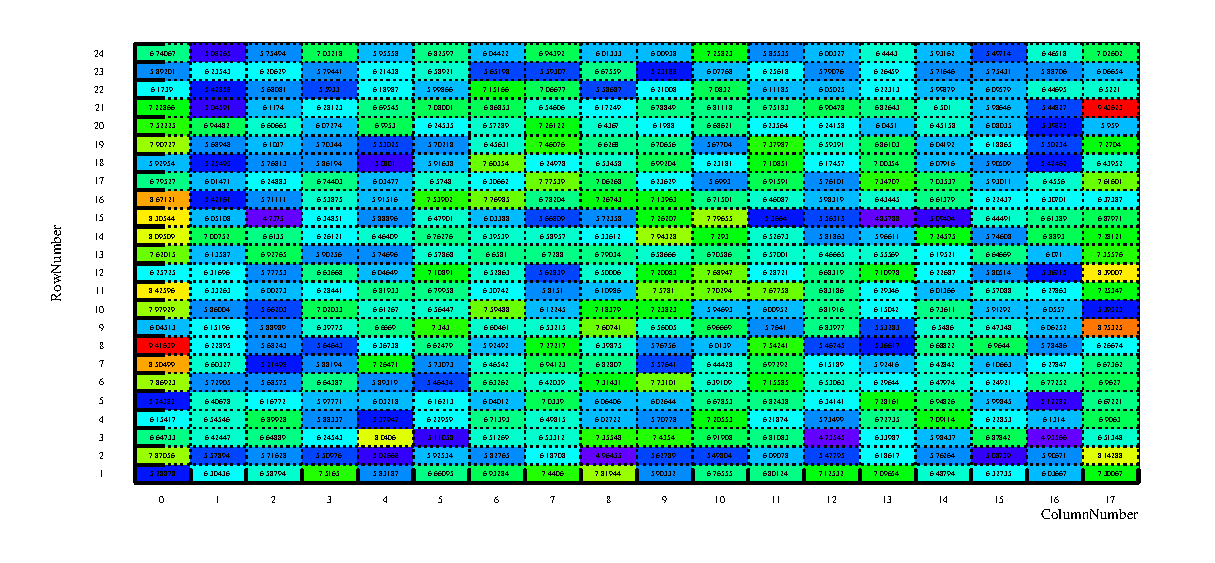
\includegraphics[width=\textwidth]{WithCollimatorScatteringRatioMerged.eps}
      \caption{\liuhao有准直器时散射的比例(\%)}
    \end{figure}
  \end{frame}
  %-----------------------------------
  \begin{frame}\frametitle{结果分析}
    \begin{minipage}[t]{0.4\textwidth}
      \liuhao
      从模拟结果来看,即使没有准直器,探测到的光子中$85\%$都是直射光子,散射光子
      比预期少了许多,原因可能有两点:
      \begin{enumerate}[1)]
	\item 一块探测器模块尺寸比模体小很多,角度稍大的散射就不能进入探测器;
	\item 入社射线束的张角为$\pm3^\circ$,集中在中心轴线附近,这部分物质较多,
	  吸收很多;
      \end{enumerate}
      用右下图的探测器模型很容易验证1),同样以张角为$\pm3^\circ$入射,这时候探测到
      的散射光子数增加到44\%。
    \end{minipage}
    \begin{minipage}[t]{0.58\textwidth}
      \begin{figure}[ht]
	\centering
	\includegraphics[width=0.8\textwidth,height=0.4\textwidth]{targetVSdetector.png}

	\includegraphics[width=0.8\textwidth]{tubdetector.png}
	\caption{\liuhao 模体与探测器模块}
      \end{figure}
    \end{minipage}
  \end{frame}
%=========================================
  \ThankYouPage
\end{CJK*}
\end{document}
